\documentclass{article}

\usepackage[italian]{babel}
\usepackage[margin=2cm, footskip=5mm]{geometry}
% questi package non sono necessari in lualatex; ref https://tex.stackexchange.com/a/413046
% \usepackage[utf8]{inputenc}
% \usepackage[T1]{fontenc}
\usepackage{enumitem}
\usepackage{hyperref}
\usepackage{titlesec}
\usepackage{soulutf8}
\usepackage{contour}
\usepackage{float}
\usepackage{graphicx}
\usepackage{fancyhdr}
\usepackage{longtable}
\usepackage[table]{xcolor}
\usepackage{titling}
\usepackage{lastpage}
\usepackage{ifthen}
\usepackage{calc}
\usepackage{minted}
\usepackage{pgfgantt}
\usepackage{subfiles}

\newlength{\imgwidth}

\newcommand\scalegraphics[1]{%
    \settowidth{\imgwidth}{\includegraphics{#1}}%
    \setlength{\imgwidth}{\minof{\imgwidth}{\textwidth}}%
    \includegraphics[width=\imgwidth]{#1}%
}

% XXX definizione dei percorsi in cui cercare immagini
\graphicspath{ {./}
    {./img/}
}

% esempio di utilizzo: \appendToGraphicspath{./img/} (un comando diverso per ogni path da includere)
% N.B.: ci DEVE essere un forward slash alla fine del path, a indicare che è una cartella.
\makeatletter
\newcommand\appendToGraphicspath[1]{%
  \g@addto@macro\Ginput@path{{#1}}%
}
\makeatother

% setup della sottolineatura
\setuldepth{Flat}
\contourlength{0.8pt}

\newcommand{\uline}[1]{%
  \ul{{\phantom{#1}}}%
  \llap{\contour{white}{#1}}%
}

% setup dei link
\hypersetup{
  colorlinks=true, % set true if you want colored links
  linktoc=all,     % set to all if you want both sections and subsections linked
  linkcolor=black, % choose some color if you want links to stand out
}

% setup di header e footer
\pagestyle{fancy}

\fancyhf{}
\fancyhead[L]{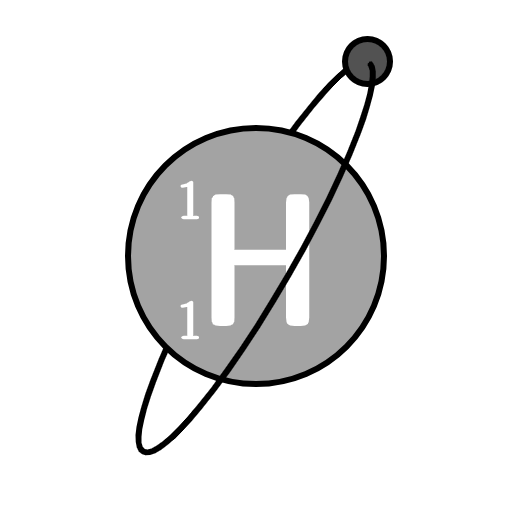
\includegraphics[width=1cm]{logo.png}}
\fancyhead[R]{\thetitle}
\fancyfoot[R]{\thepage\ di~\pageref{LastPage}}

\fancypagestyle{nopage}{%
  \fancyfoot{}%
}

\setlength{\headheight}{1.2cm}

% setup forma \paragraph e \subparagraph
\titleformat{\paragraph}[hang]{\normalfont\normalsize\bfseries}{\theparagraph}{1em}{}
\titleformat{\subparagraph}[hang]{\normalfont\normalsize\bfseries}{\thesubparagraph}{1em}{}

% setup profondità indice di default
\setcounter{secnumdepth}{5}
\setcounter{tocdepth}{5}

% shortcut per i placeholder
\newcommand{\plchold}[1]{\textit{\{#1\}}} % chktex 20

% hook per lo script che genera il glossario
\newcommand{\glossario}[1]{\underline{#1}\textsubscript{g}}

% definizione dei comandi \uso e \stato
\makeatletter
\newcommand{\setUso}[1]{%
  \newcommand{\@uso}{#1}%
}
\newcommand{\uso}{\@uso}

\newcommand{\setStato}[1]{%
  \newcommand{\@stato}{#1}%
}
\newcommand{\stato}{\@stato}

\newcommand{\setVersione}[1]{%
  \newcommand{\@versione}{#1}%
}
\newcommand{\versione}{\@versione}

\newcommand{\setResponsabile}[1]{%
  \newcommand{\@responsabile}{#1}%
}
\newcommand{\responsabile}{\@responsabile}

\newcommand{\setRedattori}[1]{%
  \newcommand{\@redattori}{#1}%
}
\newcommand{\redattori}{\@redattori}

\newcommand{\setVerificatori}[1]{%
  \newcommand{\@verificatori}{#1}%
}
\newcommand{\verificatori}{\@verificatori}

\newcommand{\setDescrizione}[1]{%
  \newcommand{\@descrizione}{#1}%
}
\newcommand{\descrizione}{\@descrizione}

\newcommand{\setModifiche}[1]{%
  \newcommand{\@modifiche}{#1}%
}

\newcommand{\modifiche}{\@modifiche}

\makeatother

% setup delle description
\setlist[description,1]{font=$\bullet$\hspace{1.5mm}, labelwidth=* leftmargin=*,labelindent=12.5mm}
\setlist[description,2]{font=$\bullet$\hspace{1.5mm}, leftmargin=*,labelindent=12.5mm}

\appendToGraphicspath{../../commons/img/}

\begin{document}
\section{Pianificazione}%
\label{sec:pianificazione}
\subsection{Pianificazione architetturale}%
\label{sub:pianificazione_architetturale}
\subsubsection{Integrazione in uscita dalla rr}%
\label{subs:integrazione_in_uscita_dalla_rr}
Date corrette: 22/01/2020 \symbol{8594} 04/02/2020.
% subs:integrazione_in_uscita_dalla_rr (end)
\subsubsection{Progettazione architetturale}%
\label{subs:progettazione_architetturale}
Date corrette: 05/02/2020 \symbol{8594} 09/03/2020.
% subs:progettazione_architetturale (end)
% sub:pianificazione_architetturale (end)
% sec:pianificazione (end)
\section{Preventivo}%
\label{sec:preventivo}
\subsection{Fase di progettazione architetturale}%
\label{sub:fase_di_progettazione_architetturale}
\begin{table}[H]
  \centering
  \rowcolors{2}{lightgray}{white!80!lightgray!100}
  \renewcommand{\arraystretch}{2}
  \begin{tabular}{c c c c c c c c}
    \rowcolor{darkgray!90!}\color{white}{\textbf{Componente}} & \color{white}{\textbf{Re}} & \color{white}{\textbf{Am}} & \color{white}{\textbf{An}} & \color{white}{\textbf{Pt}} & \color{white}{\textbf{Pr}} & \color{white}{\textbf{Ve}} & \color{white}{\textbf{Totali per persona}} \\
    Agatea Riccardo&5&-&-&10&8&5&28\\
    Apolloni Tobia&-&-&-&8&10&10&28\\
    Cestaro Riccardo&-&-&5&8&10&5&28\\
    Cocco Alberto&-&5&-&10&8&5&28\\
    Ercole Luca&-&5&-&10&8&5&28\\
    Gobbo Alberto&-&-&5&8&10&5&28\\
    Rizzo Alessandro&5&-&-&10&8&5&28\\
    Scettro Fabio&-&-&-&8&10&10&28\\
    Totali per ruolo&10&10&10&72&72&50&224\\
  \end{tabular}
  \caption{prospetto orario per la progettazione architetturale}%
~~\label{tab:prospetto_orario_progettazione_architetturale}
\end{table}
\begin{table}[H]
  \centering
  \rowcolors{2}{lightgray}{white!80!lightgray!100}
  \renewcommand{\arraystretch}{2}
  \begin{tabular}{c c c}
    \rowcolor{darkgray!90!}\color{white}{\textbf{Ruolo}} & \color{white}{\textbf{Totale ore}} & \color{white}{\textbf{Costo}} \\
    Re&10&300,00€\\
    Am&10&200,00€\\
    An&10&250,00€\\
    Pt&72&1 584,00€\\
    Pr&72&1 080,00€\\
    Ve&50&750,00€\\
    \textbf{Totale}&224&4 164,00€\\
  \end{tabular}
  \caption{prospetto economico per la progettazione architetturale}%
~~\label{tab:prospetto_economico_progettazione_architetturale}
\end{table}
% sub:fase_di_progettazione_architetturale (end)
\subsection{Totali}%
\label{sub:totali}
\subsubsection{Totali complessivi}%
\label{subs:totali_complessivi}
\begin{table}[H]
  \centering
  \rowcolors{2}{lightgray}{white!80!lightgray!100}
  \renewcommand{\arraystretch}{2}
  \begin{tabular}{c c c c c c c c}
    \rowcolor{darkgray!90!}\color{white}{\textbf{Componente}} & \color{white}{\textbf{Re}} & \color{white}{\textbf{Am}} & \color{white}{\textbf{An}} & \color{white}{\textbf{Pt}} & \color{white}{\textbf{Pr}} & \color{white}{\textbf{Ve}} & \color{white}{\textbf{Totali per persona}} \\
    Agatea Riccardo&25&15&13&30&20&35&138\\
    Apolloni Tobia&4&15&13&40&26&40&138\\
    Cestaro Riccardo&20&13&18&26&26&35&138\\
    Cocco Alberto&8&20&27&26&22&35&138\\
    Ercole Luca&6&36&13&33&22&28&138\\
    Gobbo Alberto&8&29&18&24&24&35&138\\
    Rizzo Alessandro&25&17&13&26&22&35&138\\
    Scettro Fabio&6&29&13&28&22&40&138\\
    Totali per ruolo&102&188&114&233&184&283&1104\\
  \end{tabular}
  \caption{prospetto orario dei totali complessivi}%
~~\label{tab:prospetto_orario_totali_complessivi}
\end{table}
\begin{table}[H]
  \centering
  \rowcolors{2}{lightgray}{white!80!lightgray!100}
  \renewcommand{\arraystretch}{2}
  \begin{tabular}{c c c}
    \rowcolor{darkgray!90!}\color{white}{\textbf{Ruolo}} & \color{white}{\textbf{Totale ore}} & \color{white}{\textbf{Costo}} \\
    Re&102&3 060,00€\\
    Am&188&3 760,00€\\
    An&114&2 850,00€\\
    Pt&233&5 126,00€\\
    Pr&184&2 760,00€\\
    Ve&283&4 245,00€\\
    \textbf{Totale}&1104&21 801,00€\\
  \end{tabular}
  \caption{prospetto economico dei totali complessivi}%
~~\label{tab:prospetto_economico_totali_complessivi}
\end{table}
% subs:totali_complessivi (end)
\subsubsection{Totali rendicontati}%
\label{subs:totali_rendicontati}
\begin{table}[H]
  \centering
  \rowcolors{2}{lightgray}{white!80!lightgray!100}
  \renewcommand{\arraystretch}{2}
  \begin{tabular}{c c c c c c c c}
    \rowcolor{darkgray!90!}\color{white}{\textbf{Componente}} & \color{white}{\textbf{Re}} & \color{white}{\textbf{Am}} & \color{white}{\textbf{An}} & \color{white}{\textbf{Pt}} & \color{white}{\textbf{Pr}} & \color{white}{\textbf{Ve}} & \color{white}{\textbf{Totali per persona}} \\
    Agatea Riccardo&11&12&-&30&20&26&99\\
    Apolloni Tobia&4&12&-&26&26&31&99\\
    Cestaro Riccardo&6&10&5&26&26&26&99\\
    Cocco Alberto&8&17&-&26&22&26&99\\
    Ercole Luca&6&19&-&26&22&26&99\\
    Gobbo Alberto&8&12&5&24&24&26&99\\
    Rizzo Alessandro&11&14&-&26&22&26&99\\
    Scettro Fabio&6&12&-&28&22&31&99\\
    Totali per ruolo&60&108&10&212&184&218&792\\
  \end{tabular}
  \caption{prospetto orario dei totali rendicontati}%
~~\label{tab:prospetto_orario_totali_rendicontati}
\end{table}
\begin{table}[H]
  \centering
  \rowcolors{2}{lightgray}{white!80!lightgray!100}
  \renewcommand{\arraystretch}{2}
  \begin{tabular}{c c c}
    \rowcolor{darkgray!90!}\color{white}{\textbf{Ruolo}} & \color{white}{\textbf{Totale ore}} & \color{white}{\textbf{Costo}} \\
    Re&60&1 800,00€\\
    Am&108&2 160,00€\\
    An&10&250,00€\\
    Pt&212&4 664,00€\\
    Pr&184&2 760,00€\\
    Ve&218&3 270,00€\\
    \textbf{Totale}&792&14 904,00€\\
  \end{tabular}
  \caption{prospetto economico dei totali rendicontati}%
~~\label{tab:prospetto_economico_totali_rendicontati}
\end{table}
Il costo totale a preventivo del progetto è 14~904,00€.
% subs:totali_rendicontati (end)
% sub:totali (end)
% sec:preventivo (end)
\end{document}
